\documentclass{elsart}

\usepackage{graphicx}

\usepackage{amssymb}

\begin{document}

\section{Plotting all figures for ScenarioTest-30-c1}
\subsection{Response Time}

\begin{figure}[ht]
\centering
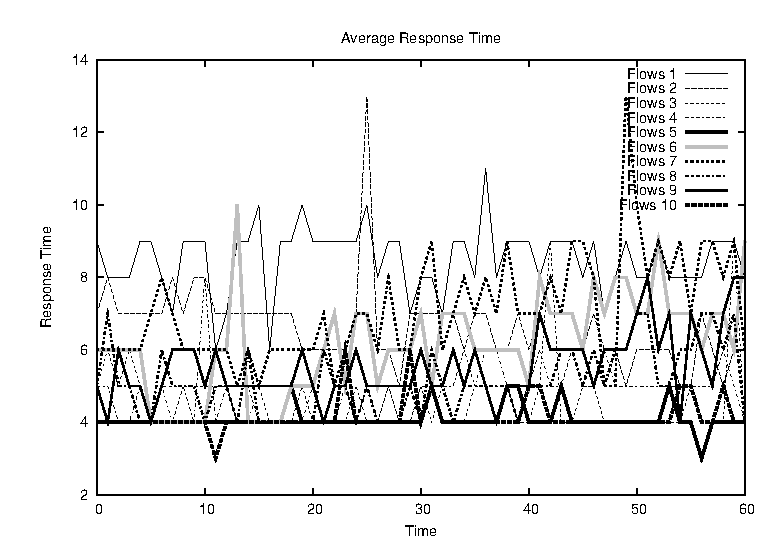
\includegraphics{ScenarioTest-30-c1/responsetime.eps}
\caption{responsetime.eps}\label{fig:responsetime}
\end{figure}

\clearpage
\subsection{Information Freshness}

\begin{figure}[ht]
\centering
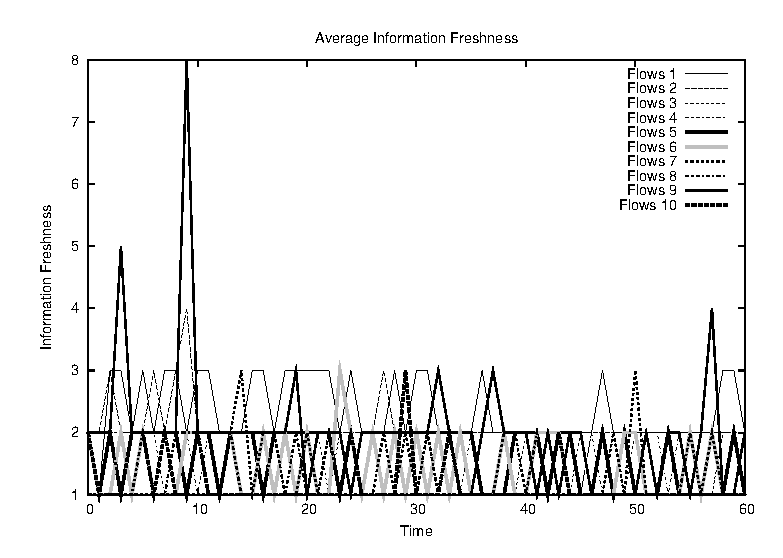
\includegraphics{ScenarioTest-30-c1/freshness.eps}
\caption{freshness.eps}\label{fig:freshness}
\end{figure}

\clearpage
\subsection{Minimum Energy Consumed}

\begin{figure}[ht]
\centering

\includegraphics{ScenarioTest-30-c1/minenergy.eps}
\caption{minenergy.eps}\label{fig:minenergy}
\end{figure}

\clearpage
\subsection{Maximum Energy Consumed}

\begin{figure}[ht]
\centering

\includegraphics{ScenarioTest-30-c1/maxenergy.eps}
\caption{maxenergy.eps}\label{fig:maxenergy}
\end{figure}

\clearpage
\subsection{Average Energy Consumed}

\begin{figure}[ht]
\centering

\includegraphics{ScenarioTest-30-c1/averageenergy.eps}
\caption{averageenergy.eps}\label{fig:averageenergy}
\end{figure}

\clearpage
\subsection{Total Energy Consumed}

\begin{figure}[ht]
\centering

\includegraphics{ScenarioTest-30-c1/totalenergy.eps}
\caption{totalenergy.eps}\label{fig:totalenergy}
\end{figure}

\clearpage
\subsection{Minimum CPU Load}

\begin{figure}[ht]
\centering
\includegraphics{ScenarioTest-30-c1/mincpuload.eps}
\caption{mincpuload.eps}\label{fig:mincpuload}
\end{figure}

\clearpage
\subsection{Maximum CPU Load}

\begin{figure}[ht]
\centering
\includegraphics{ScenarioTest-30-c1/maxcpuload.eps}
\caption{maxcpuload.eps}\label{fig:maxcpuload}
\end{figure}

\clearpage
\subsection{Average CPU Load}

\begin{figure}[ht]
\centering
\includegraphics{ScenarioTest-30-c1/averagecpuload.eps}
\caption{averagecpuload.eps}\label{fig:averagecpuload}
\end{figure}

\clearpage
\subsection{Minimum Memory Allocation}

\begin{figure}[ht]
\centering
\includegraphics{ScenarioTest-30-c1/minmemoryallocation.eps}
\caption{minmemoryallocation.eps}\label{fig:minmemoryallocation}
\end{figure}

\clearpage
\subsection{Maximum Memory Allocation}

\begin{figure}[ht]
\centering
\includegraphics{ScenarioTest-30-c1/maxmemoryallocation.eps}
\caption{maxmemoryallocation.eps}\label{fig:maxmemoryallocation}
\end{figure}

\clearpage
\subsection{Average Memory Allocation}

\begin{figure}[ht]
\centering
\includegraphics{ScenarioTest-30-c1/averagememoryallocation.eps}
\caption{averagememoryallocation.eps}\label{fig:averagememoryallocation}
\end{figure}

\clearpage
\subsection{Minimum Incoming Throughput}

\begin{figure}[ht]
\centering
\includegraphics{ScenarioTest-30-c1/minincomingthroughput.eps}
\caption{minincomingthroughput.eps}\label{fig:minincomingthroughput}
\end{figure}

\clearpage
\subsection{Maximum Incoming Throughput}

\begin{figure}[ht]
\centering
\includegraphics{ScenarioTest-30-c1/maxincomingthroughput.eps}
\caption{maxincomingthroughput.eps}\label{fig:maxincomingthroughput}
\end{figure}

\clearpage
\subsection{Average Incoming Throughput}

\begin{figure}[ht]
\centering
\includegraphics{ScenarioTest-30-c1/averageincomingthroughput.eps}
\caption{averageincomingthroughput.eps}\label{fig:averageincomingthroughput}
\end{figure}

\clearpage
\subsection{Minimum Outgoing Throughput}

\begin{figure}[ht]
\centering
\includegraphics{ScenarioTest-30-c1/minoutgoingthroughput.eps}
\caption{minoutgoingthroughput.eps}\label{fig:minoutgoingthroughput}
\end{figure}

\clearpage
\subsection{Maximum Outgoing Throughput}

\begin{figure}[ht]
\centering
\includegraphics{ScenarioTest-30-c1/maxoutgoingthroughput.eps}
\caption{maxoutgoingthroughput.eps}\label{fig:maxoutgoingthroughput}
\end{figure}

\clearpage
\subsection{Average Outgoing Throughput}

\begin{figure}[ht]
\centering
\includegraphics{ScenarioTest-30-c1/averageoutgoingthroughput.eps}
\caption{averageoutgoingthroughput.eps}\label{fig:averageoutgoingthroughput}
\end{figure}

\clearpage

\end{document}
